\documentclass[12pt, twoside]{article}
\documentclass[12pt, twoside]{article}
\usepackage[letterpaper, margin=1in, headsep=0.2in]{geometry}
\setlength{\headheight}{0.6in}
%\usepackage[english]{babel}
\usepackage[utf8]{inputenc}
\usepackage{microtype}
\usepackage{amsmath}
\usepackage{amssymb}
%\usepackage{amsfonts}
\usepackage{siunitx} %units in math. eg 20\milli\meter
\usepackage{yhmath} % for arcs, overparenth command
\usepackage{tikz} %graphics
\usetikzlibrary{quotes, angles}
\usepackage{graphicx} %consider setting \graphicspath{{images/}}
\usepackage{parskip} %no paragraph indent
\usepackage{enumitem}
\usepackage{multicol}
\usepackage{venndiagram}

\usepackage{fancyhdr}
\pagestyle{fancy}
\fancyhf{}
\renewcommand{\headrulewidth}{0pt} % disable the underline of the header
\raggedbottom
\hfuzz=2mm %suppresses overfull box warnings

\usepackage{hyperref}
\usepackage{siunitx}

\title{IB Mathematics}
\author{Chris Huson}
\date{May 2024}

%\fancyhead[LE]{\thepage}
\fancyhead[RO]{\thepage \\ Name: \hspace{1cm} \,\\}
\fancyhead[LO]{BECA/Huson/Algebra II: Regents Prep \\* 10 May 2024}

\begin{document}

\subsubsection*{Practice Regents problems \#10}
AII-F.BF.6 Represent and evaluate the sum of a finite arithmetic
or finite geometric series, using summation (sigma) notation. For geometric series:
$$\sum_{k=1}^{n} a_k = a_1 + a_2 + \ldots + a_n = a_1 \left( \frac{1-r^n}{1-r} \right)$$

\begin{enumerate}
\item Given the geometric sequence $20 \frac{1}{4}$, 27, 36, 48, $\ldots$
    %$\frac{3}{2}$, 3, $\frac{9}{2}$, 6, $\ldots$
\begin{enumerate}[itemsep=2cm]
    \item Find the common ratio $r$.
    \item Write a recursive formula for the sequence.
    \item Write an explicit formula for the sequence.
    \item Find the sum of the first 10 terms the sequence rounded to the \emph{nearest hundredth}.
\end{enumerate} \vspace{3cm}

\item Simplify each expression. 
\begin{multicols}{2}
    \begin{enumerate}
        \item $\sqrt[4]{81x^2}$
        \item $\displaystyle \frac{\sqrt[3]{x^{6}}}{\sqrt{x^{-4}}}$
    \end{enumerate}
\end{multicols}
\vspace{3cm}

\newpage
AII-F.LE.2: Construct a linear or exponential function symbolically given: a graph, a description of the relationship, or two input-output pairs (include reading these from a table).

\item Given the cubic function $f(x) = 0.2(x+2)^2(x-3)$, graphed below.
\begin{enumerate}[itemsep=1cm]
    \item State the zeros of the function.
    \item Over the interval $-2 < x < 1$, is the function increasing, decreasing, or constant?
    \item Find the average rate of change of the function over the interval from point $A$ to point $B$. \vspace{3cm}
\end{enumerate}
\begin{center}
    \begin{tikzpicture}[scale=0.5]
        \draw[lightgray,very thin] (-10,-10) grid (10,10);
        \draw [thick,<->] (-10.5,0)--(10.5,0) node [right] {$x$};
        \draw [thick,<->] (0,-10.5)--(0,10.5) node [above] {$f(x)$};
        \draw [thick,<->] plot[smooth, domain=-4.3:4.2] (\x, {0.2*(\x+2)*(\x+2)*(\x-3)});
        \fill (3,0) circle[radius=0.15] node [below right] {$A(3,0)$};
        \fill (4,7) circle[radius=0.15] node [below right] {$B(4,7)$};
    \end{tikzpicture}
    \end{center}

\end{enumerate}
\end{document}